
In the upcoming section, we will introduce basic mathematical foundations essential for the thesis. These encompass the definitions of sets, multisets, sequences, Petri nets, and event logs. We will also introduce the concept of transition systems and prefix automata. Lastly, we will provide a cursory explanation of machine learning algorithms such as Multivariable Regression as well as deep learning algorithms such as the Transformer architecture.

\begin{definition}[Set]
    A set is a collection $M$ of distinct objects. The objects in a set are called \emph{elements} of the set. The set $M$ is denoted as $M = \{ a_1, a_2, \dots, a_n \}$, where $a_1, a_2, \dots, a_n$ are the elements of the set. The notation $\lvert M \rvert$ denotes the cardinality of $M$, i.e., the number of elements in $M$.
\end{definition}

Throughout the thesis, we will use the variant $\mathbb{N} = \{0, 1, 2, \dots\}$ where $0$ is included in the set of natural numbers.

\begin{definition}[Finite Sequence]
    A finite sequence over a set $A$ is a function with the signature $\sigma \colon S \rightarrow A$ where $S = \{0, 1, \cdots, n \} \subseteq \mathbb{N}$ and $\lvert S \rvert < \infty$. The set of all finite sequences over $A$ is denoted as $A^*$. The cardinality of $S$ $\lvert S \rvert$  is the \emph{length} of a sequence $\sigma$ and is denoted it with $\lvert \sigma \rvert$.
\end{definition}

Since we are introducing the notion of sequences to represent event log traces, note that we only consider finite sequences in the scope of this thesis. Instead of the function notation, we predominantly use the list notation with angled brackets to represent sequences. For example, the sequence $\sigma \colon \{0, 1, 2, 3\} \rightarrow \{a, b, c\}, 0 \mapsto a, 1 \mapsto b, 2 \mapsto b, 3 \mapsto c$ is expressed as $\langle a, b, b, c \rangle$.

\begin{definition}[Multiset]
    A multiset over a set $A$ is a function with the signature $\mu \colon A \rightarrow \mathbb{N}$, where $\mu(a)$, $a \in A$ denotes how many times the element $a$ occurs in the multiset.  
    A multiset over a sequence $\sigma$ is a function with the signature $\mu \colon A \rightarrow \mathbb{N}$, where $\mu(a) = \lvert \{ i \mid \sigma(i) = a \} \rvert$. The set of all multisets of a set $A$ is denoted with $\mathbb{B}(A)$.
\end{definition}

Similar to sequences, we preferably use the list notation with square brackets to represent multisets rather than the function notation, where the cardinality of each element is superscripted over the element. For example, the multiset over the sequence $\langle a, b, b, c \rangle$ will be represented as $[a^1, b^2, c^1]$.

\section{Process Mining}

\textcolor{red}{TODO: Explain the basics of process mining}

\section{Event Logs}

In this section, we formally define the structure of events and event logs. Furthermore, the concept of translucent event logs is introduced.

\begin{definition}[Event]
    $\mathcal{E}$ is the event universe. An \emph{event} $e \in \mathcal{E}$ is a logical abstraction of a real-life process event. An event possesses multiple named attributes. We define the universe of all attribute names as $\mathcal{AN}$ and the universe of all attribute values as $\mathcal{AV}$.  
\end{definition}

Based on this, we define the attribute projection function $\pi \colon \mathcal{E} \times \mathcal{AN} \rightarrow \mathcal{AV} \cup \{ \perp \}$, where $\pi$ is a partial function mapping the attribute name of every event to an attribute value (otherwise a none value $\perp$). Following the convention in \cite{bible}, we denote the signature $\pi(e, n)$ as $\pi_n(e)$ for all $e \in \mathcal{E}, n \in \mathcal{AN}$.

Subsequently, a collection of events form an event log of a process.

\begin{definition}[Event Log]
    Let $\mathcal{C, A, T} \subseteq \mathcal{AV}$, where $\mathcal{C}$ is the universe of case identifiers, $\mathcal{A}$ the universe of activity names, and $\mathcal{T}$ the universe of timestamps.  An event log $\mathcal{L} \subseteq \mathcal{E}$ is a subset of the event universe such that for all events $e \in \mathcal{L}$:
    
    \begin{itemize}
        \item $\pi_{case}(e) \in \mathcal{C}$ is the case identifier,
        \item $\pi_{act}(e) \in \mathcal{A}$ is the activity name,
        \item $\pi_{time}(e) \in \mathcal{T}$ is the timestamp.
    \end{itemize}
\end{definition}

We further assume that in a conventional event log, there exists a total order $<_{time}$ on $\mathcal{L}$ such that $e <_{time} e' \iff \pi_{time}(e) < \pi_{time}(e')$ holds for all $e, e' \in \mathcal{L}$, i.e., the events are sorted by their timestamps in chronological order.

We can further group events by their case identifiers. A sequence of events with the same case identifier ordered by $<_{time}$ is called a \emph{trace}. Note that the set of all traces of an event log is pairwise disjoint, i.e., there is no event $e \in \mathcal{E}$ which is an element of two different traces. Hence, an event log can also be represented as a set of traces.

\begin{definition}[Trace]
    Let $\mathcal{E}$ be the event universe. A \emph{trace} is a sequence of events $\sigma = \langle e_1, e_2, \dots, e_n \rangle \in \mathcal{E}^*$ such that $\pi_{case}(e_i) = \pi_{case}(e_{i+1})$ holds for all $i \in \{1, \dots, n-1\}$.
\end{definition}

However, when discussing traces, we oftentimes refer to them as a sequence of activities. This is firstly for the sake of simplicity, but also due to the fact that the control flow is considered to be the most crucial aspect in process mining, in particular when constructing process models. Event logs where each trace is solely represented as a sequence of activities is called a \emph{simple event log}.

\begin{definition}[Simple Event Log]
    Let $\mathcal{L} \subseteq \mathcal{E}$ be an event log and $\sigma \in \mathcal{L}$ a trace. We expand the attribute projection function analogously for traces as the following: $\pi_n(\sigma) = \pi_n(\langle e_1, e_2, \dots, e_n \rangle) = \langle \pi_n(e_1), \pi_n(e_2), \dots, \pi_n(e_n) \rangle$. $\mathcal{L'}$ is a simple event log of $\mathcal{L}$ if
    \[
        \mathcal{L'} = \bigcup\limits_{\sigma \in \mathcal{L}} \pi_{act}(\sigma).
    \]
\end{definition}

Since we are projecting only the activity names of each event, we lose the uniqueness of each event, resulting in losing the uniqueness of each trace as well. In the simple event log setting, we therefore need to represent the event log as a multiset of traces.

The objective of our thesis is to transform conventional event logs into translucent event logs by annotating each event $e \in \mathcal{E}$ with an additional attribute $en$. $en$ specifies all activities which could have happened the moment $\pi_{act}(e)$ occurred. We formally define the notion of translucent event logs below.

\begin{definition}[Translucent Event Log]
    Let $\mathcal{L} \subseteq \mathcal{E}$ be an event log. $\mathcal{L}$ is \emph{translucent} if and only if $\pi_{en}(e) \subseteq \mathcal{A}$ and $\pi_{act}(e) \in \pi_{en}(e)$ holds for all $e \in \mathcal{L}$.
\end{definition}

Table \ref{tab:translucent_event_log} displays an example translucent event log. Note that the occurred activity in the activity column is always included in the set of enabled activities.

\renewcommand{\arraystretch}{1.25}
\begin{table}[h!]
    \centering
    \caption{Example translucent event log table.}
    \begin{tabular}{|c|c|c|c|c|c|}
        \hline
        \textbf{Case ID} & \textbf{Activity} & \textbf{Timestamp} & \textbf{Resource} & \textbf{Cost} & \textbf{Enabled Activities} \\ 
        \hline
        001 & S  & 2024-10-01 08:30 & User A & 15 & \{S\}\\ 
        001 & R    & 2024-10-01 09:00 & User B & 30 & \{R, A\}\\ 
        001 & A & 2024-10-01 09:45 & User C & 10 & \{A, F\}\\ 
        001 & E     & 2024-10-01 10:15 & User D & 5  & \{E, F\}\\ 
        001 & F & 2024-10-01 10:25 & User A & 20 & \{F\}\\
        002 & S  & 2024-10-01 11:30 & User A & 15 & \{S\}\\ 
        002 & R    & 2024-10-01 11:46 & User B & 30 & \{R, F\}\\ 
        002 & F & 2024-10-01 12:11 & User A & 10 & \{F\}\\ 
        $\vdots$ & $\vdots$ & $\vdots$ & $\vdots$ & $\vdots$ & $\vdots$ \\
        \hline
    \end{tabular}
    \label{tab:translucent_event_log}
\end{table}


\section{Automata}

In the following section, two types of automata used throughout the thesis will be defined, namely Petri nets and prefix automata.

\subsection{Petri Nets}

\begin{figure}[h!]
    \centering
    \begin{tikzpicture}[transition/.style={rectangle, draw=black, minimum width=8mm, minimum height=8mm}]
        % Define places
        \node[place, tokens=2, label=above:$p_1$] (p1) at (0, 0) {};
        \node[place, label=above:$p_2$] (p2) at (3, 1) {};
        \node[place, label=above:$p_3$] (p3) at (3, -1) {};
        \node[place, label=below:$p_4$] (p4) at (6, 0) {};
    
        \node[transition, label=below:$t_1$, right=of p1] (t1) {a}
            edge[pre] (p1)
            edge[post] (p2)
            edge[post] (p3);
        \node[transition, label=below:$t_2$, left=of p4] (t2) {b}
            edge[pre] (p2)
            edge[pre] (p3)
            edge[post] (p4);
    \end{tikzpicture}
    \caption{Example of a marked Petri net.}
    \label{fig:petrinet}
\end{figure}

Petri nets are the standard process model used in process mining, whose biggest advantage is the ability to model concurrent systems. Places of a Petri net correspond to states of a process, whereas transition of a Petri net correspond to event activities. In order to portray this behavior, we label transitions with activity names.

\begin{definition}[Petri Net]
\label{def:petrinet}
    Let $P, T$ be finite, disjoint sets, where $T$ is a set of \emph{places} and $T$ set of \emph{transitions}. A \emph{Petri net} is a triple $N = (P, T, F)$, where $F \subseteq (P \times T) \cup (T \times P)$ is a set of directed arcs between places and transitions.
\end{definition}

Figure \ref{fig:petrinet} portrays a Petri net with four places $P = \{p_1, p_2, p_3, p_4\}$, two transitions $T = \{t_1, t_2\}$, and arcs $F = \{ (p_1, t_1), (t_1, p_2), (t_1, p_3), (p_2, t_2), (p_3, t_2), (t_2, p_4) \}$. Since Petri nets are used to model the control flow of a process based on an event log, transitions should be able to represent an activity name. This is where Labeled Petri nets come into play.

\begin{definition}[Marked Labeled Petri Net]
    Let $N = (P, T, F)$ be a Petri net. A \emph{labeled Petri net} is an extended tuple $N = (P, T, F, \mathcal{A}, l)$, where $\mathcal{A}$ is a set of activity labels and $l: T \rightarrow \mathcal{A}$ is a labeling function. A \emph{marked Petri net} is an ordered pair $(N, M)$ where $M \in \mathbb{B}(P)$ is a multiset over $P$.
\end{definition}

Looking back at Figure \ref{fig:petrinet}, the transitions $t_1$ and $t_2$ are each labeled with activity names $a$ and $b$ respectively.

Furthermore, there are cases where a transition does not correspond to any of the activity names in the event log, as some are only used to model the control flow of a Petri net. These transitions are called \emph{silent transitions} (also $\tau$-transitions) and are denoted with the activity name $\tau$.

\begin{definition}[Enabled Transition]
    Let $(N, M)$ be a marked Petri net.  We further define the $\bullet$ notation, where $\pre x = \{ y \mid (y, x) \in F \}$ and $\post x= \{ y \mid (x, y) \in F \}$. A transition $t \in T$ is \emph{enabled} in $M$ if and only if $\pre t \leq M$.
\end{definition}

We also characterize this property using the notation $(N, M)[t\rangle$. The set of enabled transitions in a marked Petri net $(N, M)$ is denoted as $en(N, M) = \{ t \in T \mid \pre t \leq M \}$. An enabled transition can be \emph{fired}, which removes a token from each of its input places and adds a token to each of its output places.

\begin{definition}[Firing Rule]
    Let $(N, M)$ be a marked Petri net. The firing of a transition $t \in T$ is denoted as $(N, M) [t\rangle (N, M')$, where $M' = (M \setminus ^{\bullet}t) \cup t^{\bullet}$.
\end{definition}

Let $\sigma = \langle t_1, t_2, \dots, t_n \rangle \in T^*$ be a sequence of transitions. $(N, M)[\sigma \rangle (N, M')$ denotes that there exists a sequence of markings $\langle M_1 = M, M_2, \dots, M_{n+1} = M' \rangle$ so that \\ $(N, M_i)[t_i \rangle (N, M_{i+1})$ for all $1 \leq i \leq n$. The set of all reachable markings from $M$ is denoted as $[N, M\rangle = \{ M' \mid (N, M) [\sigma\rangle (N, M') \} \text{ for some } \sigma \in T^*$. Figure \ref{fig:firing_sequence} takes the previously defined Petri net in Figure \ref{fig:petrinet} and demonstrates the firing of a transition sequence $\langle t_1, t_2 \rangle$.

\begin{figure}[ht!]
    \centering
    \begin{subfigure}[t]{0.31\textwidth}
        % \centering
        \begin{tikzpicture}[place/.style={circle, draw=black, minimum size=6mm}]
            % Define places
            \node[place, tokens=2, label=above:$p_1$] (p1) at (0, 0) {};
            \node[place, label=above:$p_2$] (p2) at (2, 1) {};
            \node[place, label=above:$p_3$] (p3) at (2, -1) {};
            \node[place, label=above:$p_4$] (p4) at (4, 0) {};
    
            \node[transition, label=below:$t_1$, right=of p1, fill=red!50, xshift=-0.6cm] (t1) {a}
                edge[pre] (p1)
                edge[post] (p2)
                edge[post] (p3);
            \node[transition, label=below:$t_2$, left=of p4, xshift=0.6cm] (t2) {b}
                edge[pre] (p2)
                edge[pre] (p3)
                edge[post] (p4);
        \end{tikzpicture}
    \end{subfigure}
    ~
    \begin{subfigure}[t]{0.31\textwidth}
        % \centering
        \begin{tikzpicture}[place/.style={circle, draw=black, minimum size=6mm}]
            % Define places
            \node[place, tokens=1, label=above:$p_1$] (p1) at (0, 0) {};
            \node[place, tokens=1, label=below:$p_2$] (p2) at (2, 1) {};
            \node[place, tokens=1, label=above:$p_3$] (p3) at (2, -1) {};
            \node[place, label=below:$p_4$] (p4) at (4, 0) {};
    
            \node[transition, label=below:$t_1$, right=of p1, xshift=-0.6cm] (t1) {a}
                edge[pre] (p1)
                edge[post] (p2)
                edge[post] (p3);
            \node[transition, label=below:$t_2$,left=of p4, fill=red!50, xshift=0.6cm] (t2) {b}
                edge[pre] (p2)
                edge[pre] (p3)
                edge[post] (p4);
        \end{tikzpicture}
        
    \end{subfigure}
    ~
    \begin{subfigure}[t]{0.31\textwidth}
        % \centering
        \begin{tikzpicture}[place/.style={circle, draw=black, minimum size=6mm}]
            % Define places
            \node[place, tokens=1, label=above:$p_1$] (p1) at (0, 0) {};
            \node[place, label=below:$p_2$] (p2) at (2, 1) {};
            \node[place, label=above:$p_3$] (p3) at (2, -1) {};
            \node[place, tokens=1, label=below:$p_4$] (p4) at (4, 0) {};
    
            \node[transition, label=below:$t_1$, right=of p1, xshift=-0.6cm] (t1) {a}
                edge[pre] (p1)
                edge[post] (p2)
                edge[post] (p3);
            \node[transition, label=below:$t_2$, left=of p4, xshift=0.6cm] (t2) {b}
                edge[pre] (p2)
                edge[pre] (p3)
                edge[post] (p4);
        \end{tikzpicture}
    \end{subfigure}
    \caption{Firing of a transition sequence $\langle t_1, t_2 \rangle$ in an example Petri net.}
    \label{fig:firing_sequence}
\end{figure}

\begin{definition}[Lucency]
    Let $(N, M)$ be a marked Petri net. $(N, M)$ is \emph{lucent} if and only if:
    \[
        \forall M_1, M_2 \in [N, M \rangle: en(N, M_1) = en(N, M_2) \Rightarrow M_1 = M_2.
    \]
\end{definition}

As previously mentioned in \cref{chap:related_work}, \cite{sldpn} introduces an extension of a Petri net by consolidating the stochastic properties and data states into a conventional Petri net.

In a stochastic setting, the firing probability of each transition is regulated by a single weight function. If more than one transition is enabled, the transition to be fired is selected randomly based on its weights. This notion is extended even further in \cite{sldpn} by allocating a separate weight function to each transition dependent on the data states.

\begin{definition}[Stochastic Data Petri Net]
    $\Delta$ is the universe of data states. Let further $N = (P, T, F, \mathcal{A}, l)$ be a labeled Petri net. A tuple $(P, T, F, \mathcal{A}, l, \omega)$ is \emph{stochastic} if and only if $\omega: T \times \Delta \to \mathbb{R}^+$ is a weight function.
\end{definition}

Given a place $p \in P$ and a data state $\delta \in \Delta$, the probability that the Petri net $N$ fires a transition $t \in p^{\bullet}$ is given as the following equation:

\[
    Pr(t \mid p, \delta) = \frac{\omega(t, \delta)}{\sum_{t' \in p^{\bullet}} \omega(t', \delta)}.
\]

\textcolor{red}{Nur die Definition hier ist ein bisschen unverständlich, aber ein Beispiel für SLDPNs taucht eigentlich in Methods wieder auf. Soll ich hier trotzdem ein Beispiel zeigen?}

\subsection{Prefix Automata} \label{subsec:transition_systems}

\begin{definition}[Transition System]
    Let $S$ be the set of states, $A$ the set of activities, and $T \subseteq S \times A \times S$ the set of transitions. A \emph{transition system} is a triple $\mathit{\mathit{TS}} = (S, A, T)$. We denote the set of initial states as $S^{start} \subseteq S$ and the set of final states as $S^{end} \subseteq S$, where $S^{start}, S^{end} \subseteq S$.
\end{definition}

Transition systems are an alternative method next to Petri nets to represent processes of a system. Due to its structural property, silent transitions are absent in transition systems. This relieves us from the need to compute alignments when replaying the event log on the model.

\begin{definition}[Prefix Automaton]\label{def:pa}

    Let $\mathcal{L}$ be an event log and $l^{state} \colon \mathcal{L} \times \mathbb{N} \rightarrow S$ a state representation function. $\mathit{TS}_{\mathcal{L}, l^{state}} = (S, A, T)$ is a transition system based on $\mathcal{L}$ and $l^{state}$ with the following properties:
    
    \begin{itemize}
        \item $S = \{l^{state}(\sigma, k) \mid \sigma \in \mathcal{L} \land 0 \leq k \leq \lvert \sigma \rvert \}$ the state space,
        \item $A = \{ \sigma(k) \mid \sigma \in \mathcal{L} \land 1 \leq k \leq \lvert \sigma \rvert \}$ the set of activities of the event log,
        \item $T = \{ (l^{state}(\sigma, k), \sigma(k+1), l^{state}(\sigma, k+1)) \mid \sigma \in \mathcal{L} \land 0 \leq k < \lvert \sigma \rvert \}$ the set of transitions,
        \item $S^{start} = \{ l^{state}(\sigma, 0) \mid \sigma \in \mathcal{L} \}$ the set of initial states, and
        \item $S^{end} = \{ l^{state}(\sigma, \lvert \sigma \rvert) \mid \sigma \in \mathcal{L} \}$ the set of final states.
    \end{itemize} 

\end{definition}

Taking the simple event log $\mathcal{L}_1 = [ \langle a, b, c, d \rangle ^{48}, \langle a, c, b, d \rangle^2 ]$ as an example, we can construct a prefix automaton $\mathit{TS}_{L_1, hd}$ as follows:

\begin{itemize}
    \item $S = \{ \langle \rangle, \langle a \rangle, \langle a, b \rangle, \langle a, b, c \rangle, \langle a, b, c, d \rangle, \langle a, c \rangle, \langle a, c, b \rangle, \langle a, c, b, d \rangle \}$
    \item $A = \{ a, b, c, d \}$
    \item $T = \{ (\langle \rangle, a, \langle a \rangle), (\langle a \rangle, b, \langle a, b \rangle), (\langle a, b \rangle, c, \langle a, b, c \rangle), (\langle a, b, c \rangle, d, \langle a, b, c, d \rangle), (\langle a \rangle, c, \langle a, c \rangle), \\ (\langle a, c \rangle, b, \langle a, c, b \rangle), (\langle a, c, b \rangle, d, \langle a, c, b, d \rangle) \}$
    \item $S^{start} = \{ \langle \rangle \}$
    \item $S^{end} = \{ \langle a, b, c, d \rangle, \langle a, c, b, d \rangle \}$
\end{itemize}

The graphical representation is shown in Figure \ref{fig:example_prefix_automaton}.

\begin{figure}
    \centering
    \begin{tikzpicture}[->,>=stealth',shorten >=1pt,auto,node distance=2.8cm,
                        semithick]
    \tikzstyle{every state}=[fill=white,draw=black,text=black]
    
    \node[state] (<>) {$\langle \rangle$};
    \node[state] (<a>) [right of=<>] {$\langle a \rangle$};
    \node[state] (<ab>) [below right of=<a>] {$\langle a, b \rangle$};
    \node[state] (<abc>) [right of=<ab>]       {$\langle a, b, c \rangle$};
    \node[state] (<abcd>) [right of=<abc>]       {$\langle a, b, c, d \rangle$};
    \node[state] (<ac>) [above right of=<a>]       {$\langle a, c \rangle$};
    \node[state] (<acb>) [right of=<ac>]       {$\langle a, c, b \rangle$};
    \node[state] (<acbd>) [right of=<acb>]       {$\langle a, c, b, d \rangle$};
    
    \path (<>) edge node {a} (<a>)
          (<a>) edge node {b} (<ab>)
          (<a>) edge node {c} (<ac>)
          (<ab>) edge node {c} (<abc>)
          (<ac>) edge node {b} (<acb>)
          (<abc>) edge node {d} (<abcd>)
          (<acb>) edge node {d} (<acbd>);
    \end{tikzpicture}
    \caption{Example of a prefix automaton $\mathit{TS}_{L_1, hd}$ for the simple event log $\mathcal{L}_1 = [ \langle a, b, c, d \rangle ^{48}, \langle a, c, b, d \rangle^2 ]$.}
    \label{fig:example_prefix_automaton}
\end{figure}

Frequently used examples of a state representation function take the prefix function $hd^k$ as its baseline mechanism. Among diverse methods of process representation using transition systems, we focus on the list, set, and multiset representations.

\textcolor{red}{TODO: Definition für Representations verfeinern}

The set- and multiset-based representations of the prefix automaton $\mathit{TS}_{L_1, hd}$ are shown in Figures \ref{fig:example_prefix_automaton_set} and \ref{fig:example_prefix_automaton_multiset}, respectively.

\begin{figure}
    \centering
    \begin{tikzpicture}[->,>=stealth',shorten >=1pt,auto,node distance=2.8cm,
                        semithick]
    \tikzstyle{every state}=[fill=white,draw=black,text=black]
    
    \node[state] (<>) {$\{ \}$};
    \node[state] (<a>) [right of=<>] {$\{ a \}$};
    \node[state] (<ab>) [below right of=<a>] {$\{ a, b \}$};
    \node[state] (<abc>) [above right of=<ab>]       {$\{ a, b, c \}$};
    \node[state] (<abcd>) [right of=<abc>]       {$\{ a, b, c, d \}$};
    \node[state] (<ac>) [above right of=<a>]       {$\{ a, c \}$};
    \path (<>) edge node {a} (<a>)
          (<a>) edge node {b} (<ab>)
          (<a>) edge node {c} (<ac>)
          (<ab>) edge node {c} (<abc>)
          (<ac>) edge node {b} (<abc>)
          (<abc>) edge node {d} (<abcd>);
    \end{tikzpicture}
    \caption{Set-based representation of a prefix automaton $\mathit{TS}_{L_1, hd}$ for the simple event log $\mathcal{L}_1 = [ \langle a, b, c, d \rangle ^{48}, \langle a, c, b, d \rangle^2 ]$.}
    \label{fig:example_prefix_automaton_set}
\end{figure}

\begin{figure}
    \centering
    \begin{tikzpicture}[->,>=stealth',shorten >=1pt,auto,node distance=2.8cm,
        semithick]
    \tikzstyle{every state}=[fill=white,draw=black,text=black]

    \node[state] (<>) {$[]$};
    \node[state] (<a>) [right of=<>] {$[ a ]$};
    \node[state] (<ab>) [below right of=<a>] {$[ a, b ]$};
    \node[state] (<abc>) [above right of=<ab>]       {$[ a, b, c ]$};
    \node[state] (<abcd>) [right of=<abc>]       {$[ a, b, c, d ]$};
    \node[state] (<ac>) [above right of=<a>]       {$[ a, c ]$};
    \path (<>) edge node {a} (<a>)
    (<a>) edge node {b} (<ab>)
    (<a>) edge node {c} (<ac>)
    (<ab>) edge node {c} (<abc>)
    (<ac>) edge node {b} (<abc>)
    (<abc>) edge node {d} (<abcd>);
\end{tikzpicture}
    \caption{Mutliset-based representation of a prefix automaton $\mathit{TS}_{L_1, hd}$ for the simple event log $\mathcal{L}_1 = [ \langle a, b, c, d \rangle ^{48}, \langle a, c, b, d \rangle^2 ]$.}
    \label{fig:example_prefix_automaton_multiset}
\end{figure}

All these three variants have their own advantages and disadvantages. The list representation is the most precise, as it preserves the activity order of each trace. However, analyzing parallel situations is difficult due to the very same characteristics of order preservation. Moreover, the representation fails at recognizing loops in the inherent process model and is therefore susceptible to overfitting.

The set representation, on the other hand, is more general and does not suffer from order preservation issues as the list representation does. Although the property of order negligence is practical for local loops and parallel situations, it is critical for larger loops. Consider a situation with nested loops, or a loop where all activities have been already visited in the first iteration. This would lead to drastic state simplification and the resulting information loss. Here, it is crucial to select an optimal prefix length $k$.
 
The multiset representation is a compromise between the list and set representations. However, it is still not able to correctly capture the loop behavior as each iteration would create a new set of states.

\section{Machine Learning Algorithms}

In this section, we will briefly introduce and explain the machine learning algorithms employed throughout the thesis. These include Multivariable Logistic Regression, Random Forest, and the Transformer architecture.

\subsection{Multivariable Logistic Regression}

Multivariable logistic regression is a statistical model used to predict the probability of a boolean or binary outcome based on multiple variables, and is commonly applied in classification tasks. Formally, we define the model as follows:

\begin{definition}[Multivariable logistic regression]
    Given a dataset $D \in (\mathbb{R}^n \times \{0, 1\})^m$, find a function $f: \mathbb{R}^n \rightarrow [0, 1]$ such that:

    \[
        f(x) = \frac{1}{1 + e^{-\beta^T x}} \text{, where}
    \]


    \[
        \beta = \argmin_{\beta} \sum_{(x, y) \in S} \ln \left( 1  + e^{-y \beta^T x} \right).
    \]
\end{definition}

\begin{proof}
    We want to fit our regression model to the dataset $D$ as close as possible, i.e., the returned value of $f$ should be as close as possible to the binary value $y$. We therefore want to maximize:
    
    \[ \prod_{(x, y) \in S} \left(\frac{1}{ 1  + e^{-y \beta^T x}} \right). \]

    Since the function inside the product is increasing, finding the maximum of the product is equivalent to finding the maximum of the sum of its logarithm, which in turn is equivalent to finding the minimum of the negative sum of the logarithm. We can hence rewrite the term as:

    \[
        - \ln \left( \prod_{(x, y) \in S} \left(\frac{1}{ 1  + e^{-y \beta^T x}} \right) \right) = \ln \left( \prod_{(x, y) \in S} \left( 1  + e^{-y \beta^T x} \right) \right) = \sum_{(x, y) \in S} \ln \left( 1  + e^{-y \beta^T x} \right).
    \]
\end{proof}

\subsection{Random Forest}

Random Forest is an ensemble learning method that creates multiple, logically simpler decision trees and combines their predictions in order to create more accurate predictions. In contrast to conventional decision trees where the model consists of a single tree with a deep structure, Random Forests are composed of several trees with a shallow structure. The naming of the algorithm is derived from two distinct sources of randomness, namely bootstrap aggregation and random feature selection.

Bootstrap aggregation, also known as \emph{bagging}, is a dataset creation technique in which a multitude of datasets are created by sampling from the original dataset with replacement, i.e., a sample can be selected multiple times. Each of these bagged datasets is then fed to train a decision tree. Figure \ref{fig:bagging} illustrates an example of a bagged dataset.

\begin{figure}[h!]
    \centering
    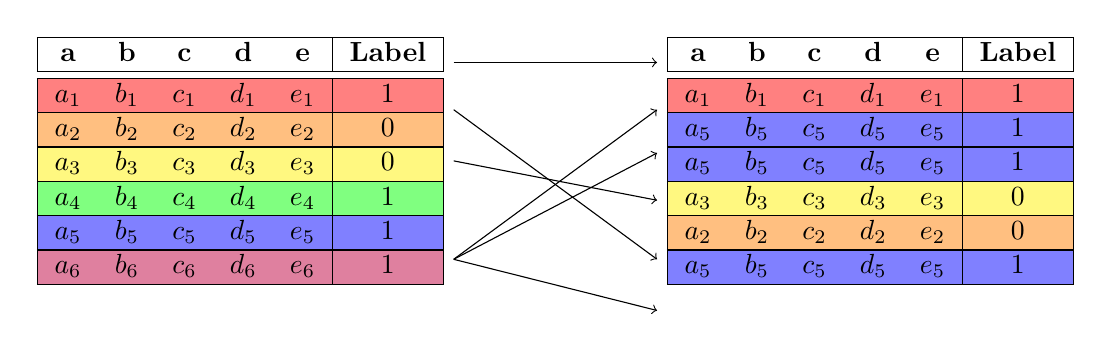
\begin{tikzpicture}

        % First table
        \node (table1) at (0,0) {
            \begin{tabular}{|ccccc|c|}
            \hline
            \textbf{a} & \textbf{b} & \textbf{c} & \textbf{d} & \textbf{e} & \textbf{Label} \\
            \hline
            \hline
            \rowcolor{red!50}
            $a_1$ & $b_1$ & $c_1$ & $d_1$ & $e_1$ & 1 \\
            \hline
            \rowcolor{orange!50}
            $a_2$ & $b_2$ & $c_2$ & $d_2$ & $e_2$ & 0 \\
            \hline
            \rowcolor{yellow!50}
            $a_3$ & $b_3$ & $c_3$ & $d_3$ & $e_3$ & 0 \\
            \hline
            \rowcolor{green!50}
            $a_4$ & $b_4$ & $c_4$ & $d_4$ & $e_4$ & 1 \\
            \hline
            \rowcolor{blue!50}
            $a_5$ & $b_5$ & $c_5$ & $d_5$ & $e_5$ & 1 \\
            \hline
            \rowcolor{purple!50}
            $a_6$ & $b_6$ & $c_6$ & $d_6$ & $e_6$ & 1 \\
            \hline
            \end{tabular}
        };
        
        % Second table
        \node (table2) at (8,0) {
            \begin{tabular}{|ccccc|c|}
                \hline
                \textbf{a} & \textbf{b} & \textbf{c} & \textbf{d} & \textbf{e} & \textbf{Label} \\
                \hline
                \hline
                \rowcolor{red!50}
                $a_1$ & $b_1$ & $c_1$ & $d_1$ & $e_1$ & $1$ \\
                \hline
                \rowcolor{blue!50}
                $a_5$ & $b_5$ & $c_5$ & $d_5$ & $e_5$ & $1$ \\
                \hline
                \rowcolor{blue!50}
                $a_5$ & $b_5$ & $c_5$ & $d_5$ & $e_5$ & $1$ \\
                \hline
                \rowcolor{yellow!50}
                $a_3$ & $b_3$ & $c_3$ & $d_3$ & $e_3$ & $0$ \\
                \hline
                \rowcolor{orange!50}
                $a_2$ & $b_2$ & $c_2$ & $d_2$ & $e_2$ & $0$ \\
                \hline
                \rowcolor{blue!50}
                $a_5$ & $b_5$ & $c_5$ & $d_5$ & $e_5$ & $1$ \\
                \hline
                \end{tabular}
        };
        
        % Draw arrows connecting the rows
        % row 1 to row 1
        \draw[->] (table1.east |- 0.5, 1.25) -- (table2.west |- 0.5, 1.25); 
        % row 5 to row 2
        \draw[->] (table1.east |- -0.5, -1.25) -- (table2.west |- 0.5, 0.65);
        % row 5 to row 3
        \draw[->] (table1.east |- -0.5, -1.25) -- (table2.west |- 0.5, 0.1);
        % row 3 to row 4
        \draw[->] (table1.east |- -0.5, 0) -- (table2.west |- 0.5, -0.5);
        % row 2 to row 5
        \draw[->] (table1.east |- -0.5, 0.65) -- (table2.west |- 0.5, -1.25);  
        % row 5 to row 6
        \draw[->] (table1.east |- -0.5, -1.25) -- (table2.west |- 0.5, -1.9);  
        
        \end{tikzpicture}
    \caption{Example of bagging. Each row is randomly selected from the original dataset. Sampling with replacement is clearly visible through multiple instances of the fifth row.}
    \label{fig:bagging}
\end{figure}

The term random feature selection refers to the procedure of utilizing a randomly selected subspace of the feature space when finding the optimal split at a decision tree's node. This method is reported to improve the model's accuracy and make the model less prone to outliers \cite{random-forest-breiman}. Figure \ref{fig:random-feature-selection} demonstrates the process of random feature selection.


\begin{figure}[h!]
    \centering
    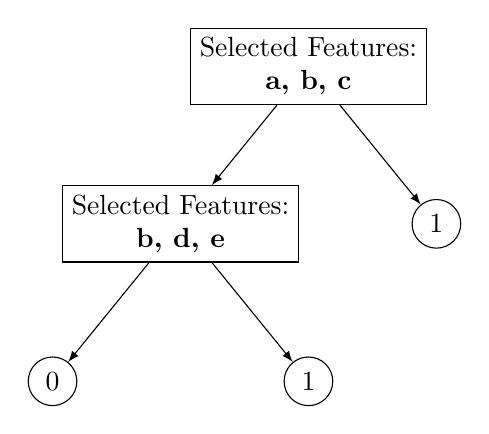
\begin{tikzpicture}[level distance=2cm,
        sibling distance=3.25cm, edge from parent/.style={draw,-latex}]
        
        % Root node
        \node[draw, rectangle, align=center] {Selected Features: \\ \textbf{a, b, c}}
            child {
                node[draw, rectangle, align=center] {Selected Features: \\ \textbf{b, d, e}}
                child { node[draw, circle, align=center] {0} }
                child { node[draw, circle, align=center] {1} }
            }
            child {
                node[draw, circle, align=center] {1}
            };
            
    \end{tikzpicture}
    \caption{Illustration of random feature selection.}
    \label{fig:random-feature-selection}
\end{figure}

After the set of decision trees is trained, the model then aggregates the predictions of individual trees to compute the final prediction. This is done by, e.g., taking a majority vote of the prediction among the set of trees. For a deeper theoretical background, we refer to the papers \cite{random-forests-ho} and \cite{random-forest-breiman}.

\subsection{Transformer Architecture}

Compared to earlier models such as RNNs or LSTMs mentioned in \cref{chap:related_work}, the transformer is a newer form of architecture first introduced in 2017 with \cite{attention-is-all-you-need}. The centerpiece of transformers is the self-attention mechanism, enabling the model to express interdependent semantic context between word tokens.

When given an input sequence, the transformer first splits up the input sequence into word embeddings known as tokens. Each token $t_i$ is then multiplied with parameter matrices $W^Q, W^K, W^V$ in order to obtain its query, key, and value vectors $q_i, k_i, v_i$ respectively. Note that the parameter matrices are learned during the training phase. 

For each token $t_i$, we then compute the attention score w.r.t. all other tokens in the sequence by taking the dot product of the query vector $q_i$ and the key vector of all tokens $k_1, \cdots, k_n$. The scalar product is also described as the \emph{compatibility function} of the query-key pairs. The attention scalar is ultimately employed as weights for the value vectors $v_1, \cdots, v_n$, whose weighted sum is a representation of $t_i$ where the contextual information of peer tokens are imputed. 


It is often characterized by the equation

\newcommand*{\vertbar}{\rule[-1ex]{0.5pt}{2.5ex}}
\[
    \text{Attention}(Q, K, V) = \text{softmax} \left( \frac{QK^T}{\sqrt{d_k}} \right) V, \text{ where}
\]

\[
    Q = 
    \left(
      \begin{array}{@{\hskip 2pt}c@{\hskip 4pt}c@{\hskip 4pt}c@{\hskip 4pt}c@{\hskip 2pt}}
        \vertbar & \vertbar &        & \vertbar \\
        q_{1}    & q_{2}    & \ldots & q_{n}    \\
        \vertbar & \vertbar &        & \vertbar 
      \end{array}
    \right), 
    K = 
    \left(
    \begin{array}{@{\hskip 2pt}c@{\hskip 4pt}c@{\hskip 4pt}c@{\hskip 4pt}c@{\hskip 2pt}}
        \vertbar & \vertbar &        & \vertbar \\
        k_{1}    & k_{2}    & \ldots & k_{n}    \\
        \vertbar & \vertbar &        & \vertbar 
    \end{array}
    \right),
    V = 
    \left(
    \begin{array}{@{\hskip 2pt}c@{\hskip 4pt}c@{\hskip 4pt}c@{\hskip 4pt}c@{\hskip 2pt}}
        \vertbar & \vertbar &        & \vertbar \\
        v_{1}    & v_{2}    & \ldots & v_{n}    \\
        \vertbar & \vertbar &        & \vertbar 
    \end{array}
    \right)
\]

are the query, key, and value matrices, respectively containing the query, key, and value vectors of each token as matrix columns, and $d_k$ is the dimension of the query and key matrices. Figure \ref{fig:self-attention} provides a graphical representation of the self-attention mechanism.

\begin{figure}[h!]

    \centering
    \begin{tikzpicture}[node distance=2cm, auto]

        % Input vectors t_1, t_2, t_3
        \node (t1) at (0,0) {$\vv{t_1}$};
        \node (t2) [below=0cm of t1] {$\vv{t_2}$};
        \node (t3) [below=0cm of t2] {$\vv{t_3}$};

        % Border around t_i
        \draw [dashed] ($(t1.north west) + (-0.10, 0.20)$)  rectangle ($(t3.south east) + (0.10, -0.20)$);

        % Query vectors q_1, q_2, q_3 with background color and border
        \node (q1) [right=1.5cm of t1, yshift=1.25cm, fill=red!30, rounded corners] {$\vv{q_1}$};
        \node (q2) [right=1.5cm of t2, yshift=1.25cm, fill=red!30, rounded corners] {$\vv{q_2}$};
        \node (q3) [right=1.5cm of t3, yshift=1.25cm, fill=red!30, rounded corners] {$\vv{q_3}$};

        % Border around q_i
        \draw [dashed] ($(q1.north west) + (-0.15, 0.15)$)  rectangle ($(q3.south east) + (0.15, -0.15)$);

        % Key vectors k_1, k_2, k_3
        \node (k1) [right=1.5cm of t1, yshift=-1.25cm, fill=green!30, rounded corners] {$\vv{k_1}$};
        \node (k2) [right=1.5cm of t2, yshift=-1.35cm, fill=green!30, rounded corners] {$\vv{k_2}$};
        \node (k3) [right=1.5cm of t3, yshift=-1.45cm, fill=green!30, rounded corners] {$\vv{k_3}$};

        % Border around k_i
        \draw [dashed] ($(k1.north west) + (-0.15, 0.15)$)  rectangle ($(k3.south east) + (0.15, -0.15)$);

        % Draw arrows from t_i to q_i & k_i
        \draw [->,>=stealth] ($(t2.east) + (3mm, 0)$) --++(0:2.5mm)|- node[near end, above] {$W^Q$} ($(q2.west) + (-3mm,0)$);
        \draw [->,>=stealth] ($(t2.east) + (3mm, 0)$) --++(0:2.5mm)|- node[near end, below] {$W^K$} ($(k2.west) + (-3mm,0)$);

        % dot product table
        \node (table) [right=3cm of t2] {
            \resizebox{4.2cm}{!}{
                \begin{tabular}{c|c|c|c|}
                    % \hline
                    $\langle \cdot \rangle$ & \tcbox[on line,left=0pt,right=0pt,top=0pt,bottom=0pt,colframe=white,colback=green!30]{$\vv{k_1}$} & \tcbox[on line,left=0pt,right=0pt,top=0pt,bottom=0pt,colframe=white,colback=green!30]{$\vv{k_2}$} & \tcbox[on line,left=0pt,right=0pt,top=0pt,bottom=0pt,colframe=white,colback=green!30]{$\vv{k_3}$} \\
                    \hline
                    \tcbox[on line,left=0pt,right=0pt,top=0pt,bottom=0pt,colframe=white,colback=red!30]{$\vv{q_1}$} & $a_{11}$ & $a_{12}$ & $a_{13}$ \\
                    \hline
                    \tcbox[on line,left=0pt,right=0pt,top=0pt,bottom=0pt,colframe=white,colback=red!30]{$\vv{q_2}$} & $a_{21}$ & $a_{22}$ & $a_{23}$ \\
                    \hline
                    \tcbox[on line,left=0pt,right=0pt,top=0pt,bottom=0pt,colframe=white,colback=red!30]{$\vv{q_3}$} & $a_{31}$ & $a_{32}$ & $a_{33}$ \\
                    \hline
                \end{tabular}
            }
        };

        % Draw arrows from q_i & k_i to table
        \draw [->,>=stealth] ($(q2.east) + (3mm, 0)$) --++(0:2.3mm)|- node[near end, above] {} ($(table.west) + (0mm,0)$);
        \draw [->,>=stealth] ($(k2.east) + (3mm, 0)$) --++(0:2mm)|- node[near end, below] {} ($(table.west) + (0mm,0)$);

        % Value vectors v_1, v_2, v_3
        \node (v1) [right=5cm of t1, yshift=-4cm, fill=blue!30, rounded corners] {$\vv{v_1}$};
        \node (v2) [right=0.1cm of v1, fill=blue!30, rounded corners] {$\vv{v_2}$};
        \node (v3) [right=0.1cm of v2, fill=blue!30, rounded corners] {$\vv{v_3}$};

        % Border around v_i
        \draw [dashed] ($(v1.north west) + (-0.15, 0.15)$)  rectangle ($(v3.south east) + (0.15, -0.15)$);
        
        % Draw arrow from t_i to v_i
        \draw [->,>=stealth] ($(t3.south) + (0, -3mm)$) |- node[very near end, above] {$W^V$} ($(v1.west) + (-3mm,0)$);

        % Resulting embeddings
        \node (e1) [right=0.3cm of table, yshift=0.35cm] {$a_{11} \cdot$ \tcbox[on line,left=0pt,right=0pt,top=0pt,bottom=0pt,colframe=white,colback=blue!30]{$\vv{v_1}$} $+ a_{12} \cdot$ \tcbox[on line,left=0pt,right=0pt,top=0pt,bottom=0pt,colframe=white,colback=blue!30]{$\vv{v_2}$} $+ a_{13} \cdot$ \tcbox[on line,left=0pt,right=0pt,top=0pt,bottom=0pt,colframe=white,colback=blue!30]{$\vv{v_3}$} $=$ \tcbox[on line,left=0pt,right=0pt,top=0pt,bottom=0pt,colframe=white,colback=yellow]{$\vv{e_1}$}};

        \node (e2) [below=-0.2cm of e1] {$a_{21} \cdot$ \tcbox[on line,left=0pt,right=0pt,top=0pt,bottom=0pt,colframe=white,colback=blue!30]{$\vv{v_1}$} $+ a_{22} \cdot$ \tcbox[on line,left=0pt,right=0pt,top=0pt,bottom=0pt,colframe=white,colback=blue!30]{$\vv{v_2}$} $+ a_{23} \cdot$ \tcbox[on line,left=0pt,right=0pt,top=0pt,bottom=0pt,colframe=white,colback=blue!30]{$\vv{v_3}$} $=$ \tcbox[on line,left=0pt,right=0pt,top=0pt,bottom=0pt,colframe=white,colback=yellow]{$\vv{e_2}$}};

        \node (e3) [below=-0.2cm of e2] {$a_{31} \cdot$ \tcbox[on line,left=0pt,right=0pt,top=0pt,bottom=0pt,colframe=white,colback=blue!30]{$\vv{v_1}$} $+ a_{32} \cdot$ \tcbox[on line,left=0pt,right=0pt,top=0pt,bottom=0pt,colframe=white,colback=blue!30]{$\vv{v_2}$} $+ a_{33} \cdot$ \tcbox[on line,left=0pt,right=0pt,top=0pt,bottom=0pt,colframe=white,colback=blue!30]{$\vv{v_3}$} $=$ \tcbox[on line,left=0pt,right=0pt,top=0pt,bottom=0pt,colframe=white,colback=yellow]{$\vv{e_3}$}};

        % Draw arrow from table to e_2
        \draw [->,>=stealth] ($(table.east) + (0, -0.36)$) -- (e2.west);

        % Draw arrow from v_i to e_i
        \draw [->,>=stealth] ($(v3.east) + (3mm, 0)$) -| ($(e3.south) + (0,0)$);

        % Border around e_i
        \draw [dashed] ($(e1.north east) + (-0.05, 0.15)$)  rectangle ($(e3.south east) + (-0.85, -0.15)$);
    \end{tikzpicture}
    \caption{An example illustration of the self-attention mechanism with three input tokens.}
    \label{fig:self-attention}

\end{figure}










For further reference, the definitive paper on transformer models is \cite{attention-is-all-you-need}.




\begin{comment}
    \begin{definition}[Directly-Follows Graph]
    
\end{definition}

\begin{definition}[Finally-Follows Graph]
    
\end{definition}

\begin{definition}[Non-local dependency]
    
\end{definition}

\begin{definition}[Mining Non-local dependencies]
    
\end{definition}

\end{comment}



\begin{comment}
    Limitations of translucent logs: Cannot solve the problem of non-local dependencies, as there are non-free-choice nets that are not lucent. However: Translucent event logs function as a safeguard to differentiate non-local dependencies from the local dependencies in a potentially incomplete event log.
\end{comment}
